% The runtime state machine. Built once (make figures) into fsm.pdf, which the
% report includes at \textwidth and the README shows as PNG and SVG.
% Nodes are placed here; every edge comes from reports/generated/fsm_edges.tex,
% which scripts/sync_docs.py writes from state.TRANSITIONS.
\pdfinfoomitdate=1
\pdftrailerid{}
\pdfsuppressptexinfo=-1
\documentclass[border=0pt]{standalone}
\usepackage{mathptmx}
\usepackage{courier}
\usepackage{tikz}
\usetikzlibrary{arrows.meta,calc,positioning}
% Shared look of the report figures: Times and Courier like the report body,
% a colour-blind-safe palette, thin dark lines.
\definecolor{statefill}{HTML}{E8EEF7}
\definecolor{verifyfill}{HTML}{DCE9F5}
\definecolor{replanfill}{HTML}{FFF2CC}
\definecolor{okfill}{HTML}{DFF0E0}
\definecolor{badfill}{HTML}{F8DEDE}
\definecolor{rejectcol}{HTML}{4477AA}
\definecolor{containcol}{HTML}{66CCEE}
\definecolor{residualcol}{HTML}{EE6677}
\definecolor{breachcol}{HTML}{222222}
\definecolor{inkcol}{HTML}{333333}
\tikzset{
  st/.style={draw=inkcol, rounded corners=2pt, fill=statefill, font=\small,
             minimum height=8mm, minimum width=16mm, inner sep=2pt},
  terminal/.style={st, double, double distance=1.2pt},
  edge/.style={-{Stealth[length=2.2mm, width=1.6mm]}, semithick, draw=inkcol},
  halo/.style={preaction={draw, white, line width=3.2pt, -}},
  lab/.style={font=\scriptsize, fill=white, inner sep=1pt, text=inkcol},
  note/.style={draw=inkcol!60, dashed, rounded corners=2pt, fill=white,
               font=\scriptsize, align=left, inner sep=3pt, text=inkcol},
  notelink/.style={dashed, draw=inkcol!60},
}

\begin{document}
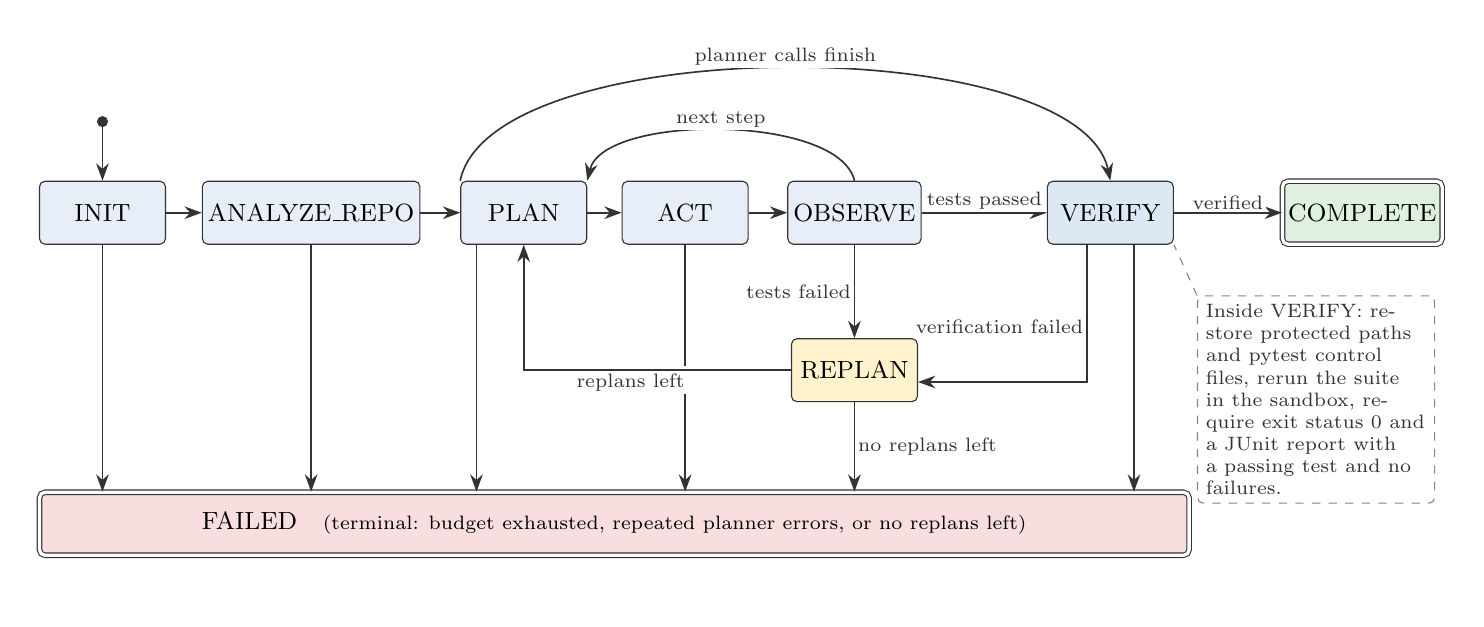
\begin{tikzpicture}[x=1cm, y=1cm]
% Exactly the report's \textwidth (516pt = 18.15cm), opaque white.
% The bottom margin also sets where the report's page 4 columns break; at
% this height both columns fill without an underfull box.
\fill[white, use as bounding box] (0,-4.90) rectangle (516pt,2.35);

\node[st] (INIT)         at (0.95,0) {INIT};
\node[st] (ANALYZE_REPO) at (3.60,0) {ANALYZE\_REPO};
\node[st] (PLAN)         at (6.30,0) {PLAN};
\node[st] (ACT)          at (8.35,0) {ACT};
\node[st] (OBSERVE)      at (10.50,0) {OBSERVE};
\node[st, fill=verifyfill] (VERIFY) at (13.75,0) {VERIFY};
\node[terminal, fill=okfill] (COMPLETE) at (16.95,0) {COMPLETE};
\node[st, fill=replanfill] (REPLAN) at (10.50,-2.0) {REPLAN};
\node[terminal, fill=badfill, minimum width=14.6cm, align=center] (FAILED) at (7.45,-3.95)
  {FAILED\quad{\scriptsize (terminal: budget exhausted, repeated planner errors, or no replans left)}};

% Start marker.
\fill[black!80] ($(INIT.north)+(0,0.75)$) circle (2pt);
\draw[edge] ($(INIT.north)+(0,0.72)$) -- (INIT.north);

% Every transition of state.TRANSITIONS.
% Generated by scripts/sync_docs.py from state.TRANSITIONS; do not edit by hand.
\draw[edge] (INIT) -- (INIT |- FAILED.north); % edge INIT -> FAILED
\draw[edge] (ANALYZE_REPO) -- (ANALYZE_REPO |- FAILED.north); % edge ANALYZE_REPO -> FAILED
\draw[edge] ([xshift=-6mm]PLAN.south) -- ([xshift=-6mm]PLAN.south |- FAILED.north); % edge PLAN -> FAILED
\draw[edge] (ACT) -- (ACT |- FAILED.north); % edge ACT -> FAILED
\draw[edge] (REPLAN) -- node[lab, right] {no replans left} (REPLAN |- FAILED.north); % edge REPLAN -> FAILED
\draw[edge] ([xshift=3mm]VERIFY.south) -- ([xshift=3mm]VERIFY.south |- FAILED.north); % edge VERIFY -> FAILED
\draw[edge] (INIT) -- (ANALYZE_REPO); % edge INIT -> ANALYZE_REPO
\draw[edge] (ANALYZE_REPO) -- (PLAN); % edge ANALYZE_REPO -> PLAN
\draw[edge] (PLAN) -- (ACT); % edge PLAN -> ACT
\draw[edge] (ACT) -- (OBSERVE); % edge ACT -> OBSERVE
\draw[edge] (OBSERVE) -- node[lab, above] {tests passed} (VERIFY); % edge OBSERVE -> VERIFY
\draw[edge] (VERIFY) -- node[lab, above] {verified} (COMPLETE); % edge VERIFY -> COMPLETE
\draw[edge] (OBSERVE.north) .. controls +(-0.2,0.85) and +(0.2,0.85) .. node[lab, above] {next step} (PLAN.north east); % edge OBSERVE -> PLAN
\draw[edge] (PLAN.north west) .. controls +(0.4,1.9) and +(-0.4,1.9) .. node[lab, above] {planner calls finish} (VERIFY.north); % edge PLAN -> VERIFY
\draw[edge] (OBSERVE) -- node[lab, left] {tests failed} (REPLAN); % edge OBSERVE -> REPLAN
\draw[edge] ([xshift=-3mm]VERIFY.south) |- node[lab, pos=0.3, left] {verification failed} ([yshift=-1.5mm]REPLAN.east); % edge VERIFY -> REPLAN
\draw[edge, halo] (REPLAN.west) -| node[lab, pos=0.3, below] {replans left} (PLAN.south); % edge REPLAN -> PLAN


% VERIFY is a state; restoring protected files is a step inside it.
\node[note, anchor=north west, text width=2.8cm] (restore) at (14.85,-1.05)
  {Inside VERIFY: restore protected paths and pytest control files, rerun
   the suite in the sandbox, require exit status 0 and a JUnit report with a
   passing test and no failures.};
\draw[notelink] (restore.north west) -- (VERIFY.south east);
\end{tikzpicture}
\end{document}
